% -/\/\/\/\/\/\/\/\/\/\/\/\/\/\/\/\/\/\/\/\/\/\/\/\/\/\/\/\/\/\/\/\/\/\/\/\/\/\/\/\/\/\/\/\/\/\/\/\/\/\/\/\/\/\/\/\/\/\/\/\/\/\/\/\/\/\/\/\/\/\/\/\/\/\/\/\/\/\/\/\/\-
%  -X-X-X-X-X-X-X-X-X-X-X-X-X-X-X-X-X-X-X-X-X-X-X-X-X-X-X-X-X-X-X-X-X-X-X-X-X-X-X-X-X-X-X-X-X-X-
% -\/\/\/\/\/\/\/\/\/\/\/\/\/\/\/\/\/\/\/\/\/\/\/\/\/\/\/\/\/\/\/\/\/\/\/\/\/\/\/\/\/\/\/\/\/\/\/\/\/\/\/\/\/\/\/\/\/\/\/\/\/\/\/\/\/\/\/\/\/\/\/\/\/\/\/\/\/\/\/\/\/-

%----------------------------------------
%----------------------------------------
\documentclass[12pt]{article}
\usepackage{geometry} 
\usepackage{indentfirst}
\usepackage{hyperref}
\usepackage{color}
\usepackage{comment}
\usepackage[pdftex]{graphicx}  
\usepackage{graphicx} 
\usepackage{caption}
\usepackage{natbib}
\usepackage{mathtools}
\usepackage{units}
\usepackage{booktabs}
\citestyle{genetics}
\renewcommand{\baselinestretch}{1.5}
\geometry{a4paper} 
\bibliographystyle{genetics}

%nouvelle commande pour les commentaires
\newcommand{\jri}[1]{\textcolor{cyan}{\bf #1}}
\newcommand{\sme}[1]{\textcolor{red}{\bf #1}}
\newcommand{\smec}[1]{\textcolor{green}{\em{\scriptsize  #1}}}
\newcommand{\com}[1]{\textcolor{blue}{ \em{\scriptsize  #1}} }

%nouvelle commande pour les suppressions 
%oh yeah, my French is awesome.
\usepackage[normalem]{ulem}
\def\dt{\bgroup
 \markoverwith{\lower-0.2ex\hbox
 {\kern-.03em\vbox{\hrule width.2em\kern0.45ex\hrule}\kern-.03em}}%
 \ULon}
\MakeRobust\dt
\usepackage[normalem]{ulem}
\def\dt{\bgroup
 \markoverwith{\lower-0.2ex\hbox
 {\kern-.03em\vbox{\hrule width.2em\kern0.45ex\hrule}\kern-.03em}}%
 \ULon}
\MakeRobust\dt

%\bibliographystyle{genetics}
%\usepackage[utf8]{inputenc} => pour les accents
%----------------------------------------
%----------------------------------------

\title{Pattern and distribution of deleterious mutations in maize}
\author{Sofiane Mezmouk and Jeffrey Ross-Ibarra} 
%\author{Sofiane Mezmouk, Robert J. Elshire, Jeffrey C. Glaubitz, \\Edward S. Buckler, and Jeffrey Ross-Ibarra}
\date{}

%-----------------------------------------------------------------------------------------------------------------
%-----------------------------------------------------------------------------------------------------------------
% BEGIN DOCUMENT
%-----------------------------------------------------------------------------------------------------------------
%-----------------------------------------------------------------------------------------------------------------
\begin{document}
\maketitle
%----------------------------------------
% ABSTRACT
%----------------------------------------
\begin{abstract} 
Amino acid changes caused by nonsynonymous single nucleotide polymorphisms may negatively impact protein function. These deleterious polymorphisms are, in general, removed by selection but may be fixed by drift or by hitchhiking with advantageous loci. To better understand the pattern of deleterious mutations in maize inbred lines, a whole genome scan for potentially deleterious amino acid polymorphisms was carried out. Using 400,000 genotyping by sequencing SNPs, in 247 maize inbred lines representative of the main genetic groups, we identified deleterious SNPs  and described their frequency along the genome and in different genetic groups.  

Nonsynonymous polymorphisms were over-represented within very low-frequency category with a large proportion being deleterious. Within the different genetic groups, very few deleterious mutations were differentially fixed. 
Association mapping with the genetic values of inbred lines and with hybrid vigor showed a small enrichment of deleterious mutations in the results; however, due to a lack of power less than half of the predicted deleterious SNPs were tested.
\end{abstract}



%----------------------------------------
% INTRODUCTION
%----------------------------------------
\newpage
\section*{Introduction}

%New mutations & Evolution
New mutations occur in every living organism. These mutations can be either neutral, with no (or very negligible) effect on fitness, or can affect individual's fitness in a given environment.

Most non-neutral mutations are disadvantageous and can even be lethal. The mutation-selection balance maintain these deleterious alleles at low frequencies. They can, however, reach moderate to high frequencies and drift to fixation if the selection pressure ($s$) is small compared to the effective population size ($s < \nicefrac{1}{2} N_{e}$; \citet{Keller2002}). Different deleterious mutations could thus be fixed in different populations or genetic groups \citep{Whitlock2003,Fay2001}.

In addition to the mutation effect and  effective population size, a number of other factors affect the destiny of deleterious alleles, such as the mating system and the recombination rate.\\
Selfing species and inbreeding within populations will expose the lethal mutations to selection faster than in an outcrossing population \citep{Keller2002}. The slightly deleterious mutations will however be maintained at moderate frequencies, even with the presence of gene flow between populations \citep{Whitlock2000}. In low recombination regions, deleterious mutations could hitchhike with advantageous alleles at linked loci \citep{Hill1966, Chun2011}. Fixation of deleterious mutations is slower with an increased recombination rate in a finite population \citep{Charlesworth1993}
 %Mutation accumulation in finite outbreeding and inbreeding populations; %D. Charlesworth, M. T. Morgan, B. Charlesworth; %Genetics Research (impact factor: 1.71). 01/1993; 61(01):39 - 56. %=>purifying selection against deleterious mutations increases the proportion of low frequency alleles and it reduces the effective population size and thus the level of neutral heterozygosity at linked loci or sites
 
%Functional variants and previous efforts
The presence of deleterious allele within loci associated to quantitative traits may explain part of there determinism and heritability. It was also suggested that complementation at deleterious SNPs could explain a non negligible part of heterosis \citep{Charlesworth2009}.\\
Evaluating the pattern of deleterious mutations is thus of interest and has been investigated in the Human genome \citep{Fay2001, Johnson2005, Lohmueller2008, Chun2009, Chun2011, Subramanian2012}, yeast \citep{Doniger2008}, bacteria \citep{Hughes2005}, RNA viruses \citep{Pybus2007} and different plant species including rice, \emph{Arabidopsis thaliana} \citep{Lu2006,Gunther2010,Cao2011}, and tomatoes \citep{Tellier2011}.

\citet{Fay2001} estimated, in 182 Human genes, the fraction of amino acid mutations that are deleterious to around 80\% with only 20\% of them being slightly deleterious. However, \citet{Johnson2005} estimated to only 20\% the variants that are damaging to the protein, in 25 genes associated with sex steroid biosynthesis. At a genome level, \citet{Lohmueller2008} observed higher proportion of SNPs predicted to be deleterious in african americans in comparison to european americans; they mainly explained this observation by the out of africa bottelneck.\\
\citet{Subramanian2012} examined the temporal pattern of deleterious SNPs at internal and terminal of the human tree in four human populations. The percentage of deleterious mutations seen reached 48\% of the amino acid variant specific to a given genome. also they observed that deleterious fraction of genome specific non synonymous SNPS is up to 7 times higher compared to that shared between human.

In a plant genome wide predictions, \citet{Gunther2010} observed different proportion of deleterious SNPs within \emph{Arabidopsis thaliana} accessions and fewer deleterious SNPs in wild rice in comparison to the cultivated accessions. Similarly, \citet{Lu2006} estimated that around 25\% of the differences between rice cultivars are deleterious. Within coding regions of eight house keeping genes, \citet{Tellier2011} estimated to 90\% the proportion of non-synonymous SNPs under selection, suggesting that they may be deleterious. 

%Maize
Maize is a worldwide economically important cereal with the highest yield and largest cultivated area within cereal  (FAO statistics, \url{http://faostat.fao.org}), distributed in a broad range of latitudes and environments \citep{Tenaillon2011} to which it adapted given its tremendous genetic diversity \citep{Chia2012}. \\
The presence of a very strong structure into heterotic groups of the maize breeding material and the high observed levels of heterosis makes it interesting to analyze the distribution of the deleterious mutations 

% what we do 
The aim of the current study was to make use of the availability of the maize genome sequence, high density single nucleotide polymorphisms (SNPs) and phenotypic data for an enough large sample of inbred lines and hybrids to (1) carry out a genome wide scan for deleterious mutations using the whole maize B73 reference genes, (2) analyze their distribution within the genome and within different genetic groups and (3) test for enrichment of these loci in the results of genome wide association mapping with both the genetic values of inbred lines and the hybrid vigor for different quantitative traits of interest.\\
Our results showed that a majority of deleterious alleles are segregating in maize; these alleles are in general at very low frequencies as expected from theory and very few are differentially fixed within different genetic groups. Genome wide association mapping results showed a small enrichment enrichment of these deleterious loci.


%----------------------------------------
% MATERIALS AND METHODS
%----------------------------------------
%\newpage
\section*{Materials and methods}
% -x-x-x-x-x-x-x-x-x-x-x-x-x-x-x-x-
\subsection*{Plant material and phenotypic data}
% -x-x-x-x-x-x-x-x-x-x-x-x-x-x-x-x-
Phenotypic data from 247 maize inbred lines from the diversity panel described by \citet{Flint-Garcia2005} were analyzed in the current study (see Supplementals for inbred line list). These inbred lines were crossed to the stiff-stalk inbred B73 (population\,A) and both the inbred lines and their B73-hybrids were evaluated in three environments in 2003 \citep{Flint-Garcia2009}. A subset of 102 inbreds were additionally crossed to both B73 (population\,B1) and Mo17 (population\,B2) and evaluated in a single environment in 2006 \citep{Flint-Garcia2009}.

Traits measured in both populations include cob diameter (cm), cob weight (g), ear length (cm), plant height (cm), individual kernel weight (g) and total kernel weight (g/ear). Additional traits including days to anthesis, plant yield (g/plant), tassel length (cm), tassel branch count, tassel angle, upper leaf angle, leaf width (cm), leaf length (cm), stem puncture resistance \com{(?kg/section)}, stem width (cm), 10 kernel weight (g) and kernel height (cm) were collected for population\,A, and seed number per ear was collected for populations B1 and B2. Details of the phenotypes and measurements can be found in \citep{Flint-Garcia2009}.

\subsection*{Genotypic data}
All 247 lines were genotyped using a genotype-by-sequencing \citep[GBS;][]{Elshire2011} approach \citep{Larsson2013}. In total, each inbred line was genotyped for partially imputed 437,650 SNPs. \smec{They did not give details about how was the imputation done}.%\jri{Missing data were partially imputed following \com{who to cite??}}
The latter were mapped to cDNAs of the first transcripts of the maize reference genome 5b filtered gene set, resulting in 259,896 SNPs mapped to 26,300 genes.  Of these, 127,994 mapped to protein coding sequences representing 123,289 codons. The median (mean) percentage of missing data per SNP, including triallelic sites, was 1.06\% (2.52\%), while the precentage of heterozygous sites was  1.08\% (2.52\%). Only 4.5\% of SNPs had more than 10\% missing data (Supp Fig~\ref{figureS1}-A), and 0.18\% had more than 10\% heterozygous genotypes (Supp Fig~\ref{figureS1}-B). The GBS data was available at \url{http://www.panzea.org/lit/data_sets.html}.

We estimated error rates by first comparing our genotyped inbred B73 to the B73 reference genome, then by comparison of all our genotypes to data from the maize SNP50 bead chip \citep{Cook2012}.  Compared to the reference genome, our B73 genotype differed at 1.75\% of SNPs, and across all lines our genotypes differ at a median (mean) rate of 1.83\% (4.62\%) of the 7,225 homozygous SNPs also present in the data of \citet{Cook2012}.   

% -x-x-x-x-x-x-x-x-x-x-x-x-x-x-x-x-
\subsection*{Statistical analyses}
% -x-x-x-x-x-x-x-x-x-x-x-x-x-x-x-x-

\subsubsection*{SNP annotation}
SNPs were annotated as synonymous and nonsynonymous using the software polydNdS from the analysis package of libsequence  \citep{Thornton2003}. The deleterious effects of amino acid changes were predicted for proteins derived from the first transcript of each gene in the B73 5.b filtered gene set \com{all correct?\smec{$\Rightarrow$yes}} using both the SIFT \citep{Ng2003, Ng2006} and MAPP \citep{Stone2005} software packages. 

SIFT uses homologous sequences identified by PSI-BLAST \com{all caps? what kind of blast does SIFT use? \smec{$\Rightarrow$PSI-BLAST}} against protein databases to identify conserved amino acids.  The software provides a scaled score of the putative deleterious effect of a particular amino acid at a position along the \sme{protein}. 

MAPP predicts deleterious amino acid polymorphisms using a user-defined alignment of protein homologs. \sme{It} uses the phylogenetic relatedness among sequences and the physicochemical properties of amino acids to quantify the potential deleterious effect of a given amino acid change. We created alignments for MAPP using three different methods.  First, we made \sme{BLASTX} %\com{need to check capitalization... e.g. BLAST or BASTX or blastx}
comparisons of protein sequences from maize against the TrEMBL database \citep{Boeckmann2003}, retaining all proteins with an e-value $\leq 10^{-40}$ and at least 60\% identity with the query.  Second, we used a reciprocal best BLAST criteria to compare protein sequences of maize against protein sequences from 31 plant genomes (see the list on Supplementals) \com{if this is a supp. table we should cite table.  otherwise can just say "supplemental data"\smec{$\Rightarrow$it's not a table}} from Phytozome version 8.0 (\url{http://www.phytozome.net}), retaining the best hit protein from each of the other genomes with a minimum e-value $\leq 10^{-100}$ \com{how to format eval. e-val? e-value?\smec{$\Rightarrow$I format it as "e-value", if you are ok}}
and covered $\geq 70\%$ of the query length. Finally, we made use of a set of syntenic genes from the grasses \emph{Zea mays}, \emph{Sorghum bicolor}, \emph{Oryza sativa} and \emph{Brachypodium distachyon}  \citep{Lyons2008}, downloaded from \url{http://synteny.cnr.berkeley.edu/CoGe/data/distrib/Supplemental_dataset_S1_pluslinks.csv}. For each set of proteins, ClustalW2 \citep{Larkin2007} was used to align the sequences and build a \sme{neighbour-joining} %\com{what kind of tree? NJ? what parameters?}
tree. An R script was used to link amino acid positions to SNP positions and to link the amino acid polymorphisms to MAPP and SIFT predictions. \com{how hard would it be to make all the R code available?  would be nice so others could replicate. \smec{$\Rightarrow$ I wrote them specifically for this context; I will think about how to make them less specific when analyzing the 12 inbreds}}

\com{please work this paragraph/data into methods. i think it's too much for results\smec{$\Rightarrow$ it's summarized on the supplementals}}
%\sme{Of the 10,532 polymorphic amino acid positions that were predicted with all three gene-sets 7,448 (70.7\%) had the same predictions for all amino acid polymorphisms with at least two gene sets; 4,469(42.4\%)  positions had the same predictions with the three gene sets. However, these comparisons are very stringent because, for a given position, if only one polymorphism is predicted differently within two different gene sets, the predictions are considered to be different.}


\subsubsection*{Phenotypic data analyses}

Genetic values of inbreds and hybrids in population\,B were taken from \citet{Flint-Garcia2009}. 
Genetic values for population A were estimated from the raw phenotypic data using the model:
%
\[Y=\mathbf{1}\mu +ZG+\varepsilon \]
%
where $Y$ is the vector of phenotypic values, $\mu$ is the mean of $Y$, $Z$ is an incidence matrix, $G$ is the vector of fixed individual effects and $\varepsilon$ are the residuals assumed to be distributed $N(0,\sigma _{\varepsilon }^{2}I)$.

Hybrid vigor for each individual was estimated by both best- and mid-parent heterosis ($BPH$ and $MPH$, respectively):
%
\[ MPH_{ij}=\hat{G_{ij}}-\frac{1}{2}(\hat{G_{i}}+\hat{G_{j}}) \]
\[ BPH_{min,ij}=\hat{G_{ij}}-min(\hat{G_{i}} ,\hat{G_{j}}) \] 
\[ BPH_{max,ij}=\hat{G_{ij}}-max(\hat{G_{i}} ,\hat{G_{j}}) \]
%
where $\hat{G_{ij}}$, $\hat{G_{i}}$ and $\hat{G_{j}}$ are the genetic values of the hybrid and its two parents $i$ and $j$. $BPH_{min}$ was used instead of $BPH_{max}$ for days to anthesis, tassel branch count, tassel angle, upper leaf angle and rind penetrometer resistance.

\subsubsection*{Association mapping}
SNP associations with the genetic values \com{sometimes you say "genotypic value" and sometimes "genetic value". i assume these are the same, but should we be consistent?\smec{$\Rightarrow$it should be genetic; I don't know why I put genotypic! sorry for that}} of the inbred lines were tested using the mixed linear model:
%
\[\hat{G}=\mathbf{1}\mu + M\vartheta +S\beta +Zu+\varepsilon\]
%
where $\hat{G}$ \sme{is the vector of} estimated genetic values \com{above for phenotypes you specify that Y is a vector.  do we need to specify that G is a vector? is it?\smec{$\Rightarrow$I changed it}} \sme{for} inbred lines, $\mu$ is the mean of $\hat{G}$, $M$ is the tested SNP, $\vartheta$ is the SNP effect, $S$ is the structure covariates estimated by \citet{Flint-Garcia2005}, $\beta$ is the fixed structure effects, $Z$ is an incidence matrix, and $u$ are the random effects assumed to be distributed as $N(0,\sigma_{ {\varepsilon}}^{2}K)$, and $\varepsilon$ are the model residuals assumed $N(0,\sigma_{ {\varepsilon}'}^{2}I)$. The coancestry matrix $K$ among inbred lines was approximated by an identity by state matrix calcu;aged with the SNPs. All SNPs used for association mapping had a minor allele frequency $\ge$ 0.05.

In hybrids, we tested the effect of heterozygosity at a given locus on observed heterosis. Each SNP was assigned numerical values corresponding to $0$ if the hybrid is homozygous or $1$ if the hybrid is heterozygous. The association mapping tests were thus carried out between heterozygosity at a given locus and hybrid vigor:
%
\[PH=\mathbf{1}{\mu}'+D\beta +H\vartheta +{\varepsilon }'\]  \com{i added boldface to 1. correct?\smec{$\Rightarrow$yes, thank you}}\\
%
where $PH$ is either $MPH$, $BPH_{max}$ or $BPH_{min}$, ${\mu}'$ is the mean of $PH$, $D$ is the genetic distance between the tester (B73 or Mo17) and each inbred line, $\beta$ is the fixed effect of that distance, $H$ is the tested locus and $\vartheta$ the effect of the locus, and ${\varepsilon }'$ is the vector of residuals assumed to be  $N(0,\sigma_{ {\varepsilon}'}^{2}I)$.  
\com{what is I? above you call $\varepsilon$ the model residuals but here you call it a vector. we should probably be consistent. \smec{$\Rightarrow$ $\varepsilon$ is a vector in both, given the matricidal writing of the equation. I is an identity matrix}}
The threshold for retained (significant) SNPs was set to $p\leq 0.001$. Furthermore, we set the false discovery rate \citep{Benjamini1995} at 10\%. 
\com{isn't setting a p-value cutoff different from using FDR? did you do both?\smec{$\Rightarrow$ I did both because we can be asked about the multiplicity problem and the FDR is a way to deal with}}

%----------------------------------------
% RESULTS AND DISCUSSION
%----------------------------------------
\section*{Results and Discussion}

% -x-x-x-x-x-x-x-x-x-x-x-x-x-x-x-x-
\subsection*{Prediction of deleterious mutations}
% -x-x-x-x-x-x-x-x-x-x-x-x-x-x-x-x-
In order to investigate deleterious mutations in a diverse set of maize inbred lines, we first made use of two complementary approaches to predict deleterious mutations across the maize genome.  We applied the software packages SIFT \citep{Ng2003, Ng2006} and MAPP \citep{Stone2005} to the 39,656 genes in version 5b of the maize filtered gene set  \citep[http://www.maizesequence.org;][]{Schnable2009}. SIFT predicted amino acid \sme{change} consequences for nearly 12 million codons in ~32,000 genes, while MAPP obtained predictions for a total of ~11 million codons in ~29,000 genes combined across the three ortholog datasets used (see methods).

We made use of genotyping-by-sequencing \citep{Elshire2011}  data to survey the diversity of potentially deleterious mutations across a large panel of \sme{diverse} maize inbred lines  \citep{Larsson2013}.\\
The genotyping data covered 112,326 and 107,472 codons representing 19,145 and 18,255 genes in the SIFT and MAPP data, respectively.  Of these, in each dataset \sme{nearly 50}\% showed no amino acid polymorphism. While the vast majority of these monomorphic amino acids were due to synonymous polymorphisms in the GBS data, several hundred putatively deleterious amino acids were fixed across all maize lines analyzed (Supplemental Table~\ref{tableS1}).\\
Among the codons covered by GBS SNPs, predictions were made by both SIFT and MAPP for 20,195 genes (95\%). More than 80\% of predictions were congruent between the two approaches; an overlap similar to what has been seen in \emph{Arabidopsis thaliana} and rice \citep{Gunther2010}.

SIFT and MAPP identified, respectively, ~80\%  and 60 \% of amino acid polymorphisms as ``tolerated", with the remainder predicted to be premature stop codons or ``non-tolerated" amino acid changes. \com{ don't both programs give numeric rankings of effect? could we show a graph of those? might be interesting?\smec{$\Rightarrow$ they do. I already tried the plots and they are not very nice; I am happy to redo them if you want to check them}}

\com{I think a good way to show these data would be a venn diagram in the supp.  you could have two. one would show three approaches for MAPP (to be cited in methods), and the other MAPP and SIFT. thoughts? am i correct that in the final data you had 53,252 poymorphic predictions for SIFT and of those 46,741 were also in MAPP?  How many MAPP were not in SIFT? that could be in Venn diagram.\smec{$\Rightarrow$ Ok; I will summarize all the text you put as comments in Venn diagrams etc ...}}

% Figure1
%-------------------------------------------------------------------
\begin{figure*}[ht]
  \begin{center}
   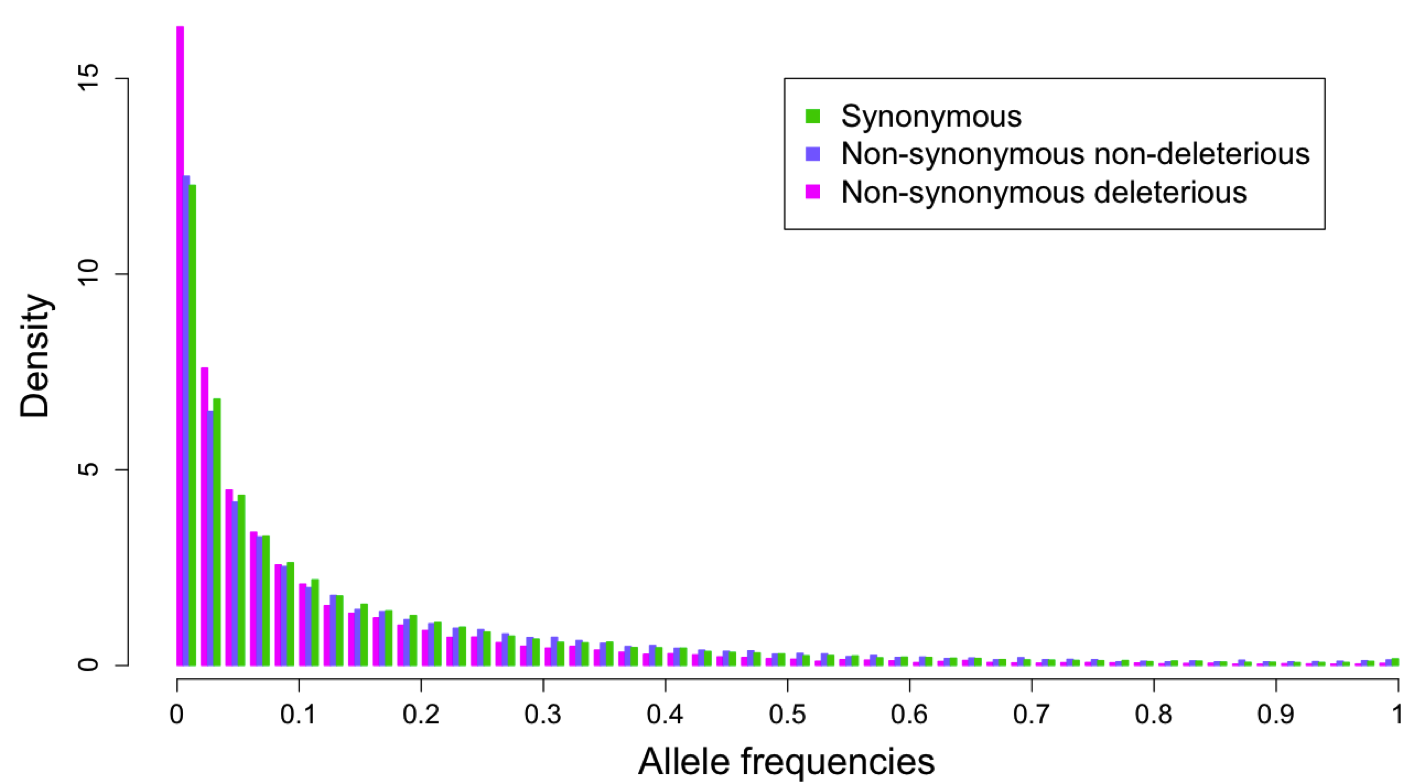
\includegraphics[width=150mm]{SFS.png}
    \caption{Site frequency spectrum of (A) synonymous \emph{vs} non synonymous SNPs and (b) non-synonymous non-deleterious \emph{vs} non-synonymous deleterious SNPs} \com{Maybe make the graphs a bit bigger.  Hard to see the light blue and light grey.  Or maybe make them white w/ black outline and grey fill?  not sure, we can try options but these are a bit hard to read at this size. fst one (fig. 3) is a bit better, but still hard at that size.  maybe as density plots?  thoughts?\smec{$\Rightarrow$ I changed the plot I have them with 0.02 and 0.05 break points}}
   \label{sfs_non_syn}
  \end{center}
\end{figure*}
%-------------------------------------------------------------------


% -x-x-x-x-x-x-x-x-x-x-x-x-x-x-x-x-
\subsection*{Characterization of deleterious SNPs in a diversity panel}
% -x-x-x-x-x-x-x-x-x-x-x-x-x-x-x-x-

\com{nowhere do we have analysis of strongly deleterious vs. weakly.  we get quantitative information from MAPP and SIFT, right? are there interesting differences in strong vs. weak predicted deleterious mutations?}

%general SFS
The site frequency spectrum of protein-coding SNPs showed an excess of rare variants compared to neutral expectations , with 45\% of SNPs at a frequency lower than 5\% across all lines.  \com{this refers to all SNPs correct?\smec{$\Rightarrow$ yes}} Among these low frequency SNPs an excess of nonsynonymous SNPs was observed (\sme{Mann-Whitney U test p-value $< 2.2\ 10^{-16}$} ; Figure~\ref{sfs_non_syn}-A).  Deleterious SNPs, making up a combined 22\% of all protein coding SNPs, showed an even more marked excess of rare variants (\sme{Mann-Whitney U test p-value $< 2.2\ 10^{-16}$} ; Figure~\ref{sfs_non_syn}-B). \com{in all three cases a MW U test might be good to show significance?\smec{$\Rightarrow$ I added it}} These observations are consistent with the action of purifying selection acting against deleterious alleles  \citep{Fay2001} and provide independent corroboration of the utility of MAPP and SIFT in predicting deleterious variants.

\sme{Working on the Haplotype test; sill update the following paragraph as soon as it finishes running}\\
Although, most \sme{predicted} \com{ not a fan of putative? we can use predicted, potential, etc.\smec{$\Rightarrow$ ok I will go with predicted; I replaced all putative}} deleterious alleles were rare, 922 were found at high frequencies ($\geq 0.80$) . To test whether these alleles may in fact represent functional amino acid changes affected by positive selection, we did XYZ \com{please elaborate on haplotype test and comparison with genes from Matt's paper\smec{$\Rightarrow$I did it but the results are not interesting; I am happy to show them to you}. should probably add at least hap test or both to methods\smec{$\Rightarrow$I will add the hap test}}.  These analyses fail to find evidence of positive selection \com{rewrite/explain findingds}, suggesting ABC \com{explanation for these? drift? error?\smec{$\Rightarrow$ ok; I will finish that}}.

%per line SNPs

Individual lines varied considerably in their \sme{content} of predicted deleterious alleles, carrying between 4 and 16\% of all predicted deleterious alleles.\\
\com{should cite some sup. table/figure. do we need to correct for avg. content of minor alleles in a line? migth be nice to identify lines with more or less del. alleles than we expect based on minor alleles at syn sites? or is this silly? \smec{$\Rightarrow$ please check the plot"CorrNbDelvsNbRare.pdf", the correlation is high but not linearity's one value per inbred}} \\
Lines from the stiff stalk heterotic group carried, on average, fewer deleterious mutations (9\%) than did lines from other groups (14-15\%).  While this may be due to the historically smaller $N_{e}$ of the stiff stalk group \sme{\citep{Messmer1991}}, other groups with historically small $N_{e}$ such as the popcorns do not show such a trend; this result may instead arise due to biases in prediction using the stiff stalk line B73 reference genome.
% find this paper Lamkey, K.R. 1992. Fifty years of recurrent selection in the Iowa Stiff Stalk Synthetic maize population. Maydica 37:19�28. for the founders of the stiff stalk

%overall IBS, shared alleles

Allele sharing at predicted deleterious SNPs closely mirrored that of overall identity by state (IBS)\sme{, approximated by the percentage of shared SNPs}. \com{how is IBS measured? SNP by SNP or haplotypes or?\smec{$\Rightarrow$ SNP by SNP}} \\
Within heterotic groups, correlations were generally high (Pearson $r$ of 0.75-0.99) \com{what do these numbers represent? means? do they include the 0.15 for SS? \smec{$\Rightarrow$ value of the correlation between IBS and \% of shared deleterious in each gouts; does not include the SS and mixed}} between numbers of shared deleterious alleles (mean of 5 -10\%) and IBS.  Correlations for inbreds from different genetic groups were much lower ($r$ of 25 - 52 \%) than that observed within the same group. Both patterns mimic correlations seen between IBS and heterosis which are higher for the inbred lines from the tester heterotic group compared to the correlations with the other inbred line. This pattern was previously observed with SSRs \citep{Flint-Garcia2009}. \com{ could we recalculate this correlation? we have better IBS data than they did don't we?} The "mixed" (within group $r=0.22$, $r=-0.05\ to\ 0.36$ with the other groups) and stiff stalk (within-group $r=0.15$, $r=-0.65\ to\ 0.16$ with the other groups) groups appeared to be exceptions to this rule, perhaps due to unrecognized population substructure within these groups \sme{as suggested by a PCA within these groups (Supplemental Figure~\ref{figureS3})}. 
\smec{The pattern would suggest 3 subgroups in the ss$\Rightarrow$ check if it fits Iodent, RYD and pure SS subgroups} \com{where does the result of 3 subgroups come from? PCA? Flint-Garcia? i think if we make this argument (i believe it) we need some supp. data to back it up?\smec{$\Rightarrow$ I did the PCA intra-group; it corroborates what I was thinking}} 

% Fst

% Figure2
%-------------------------------------------------------------------
\begin{figure*}[ht]
  \begin{center}
   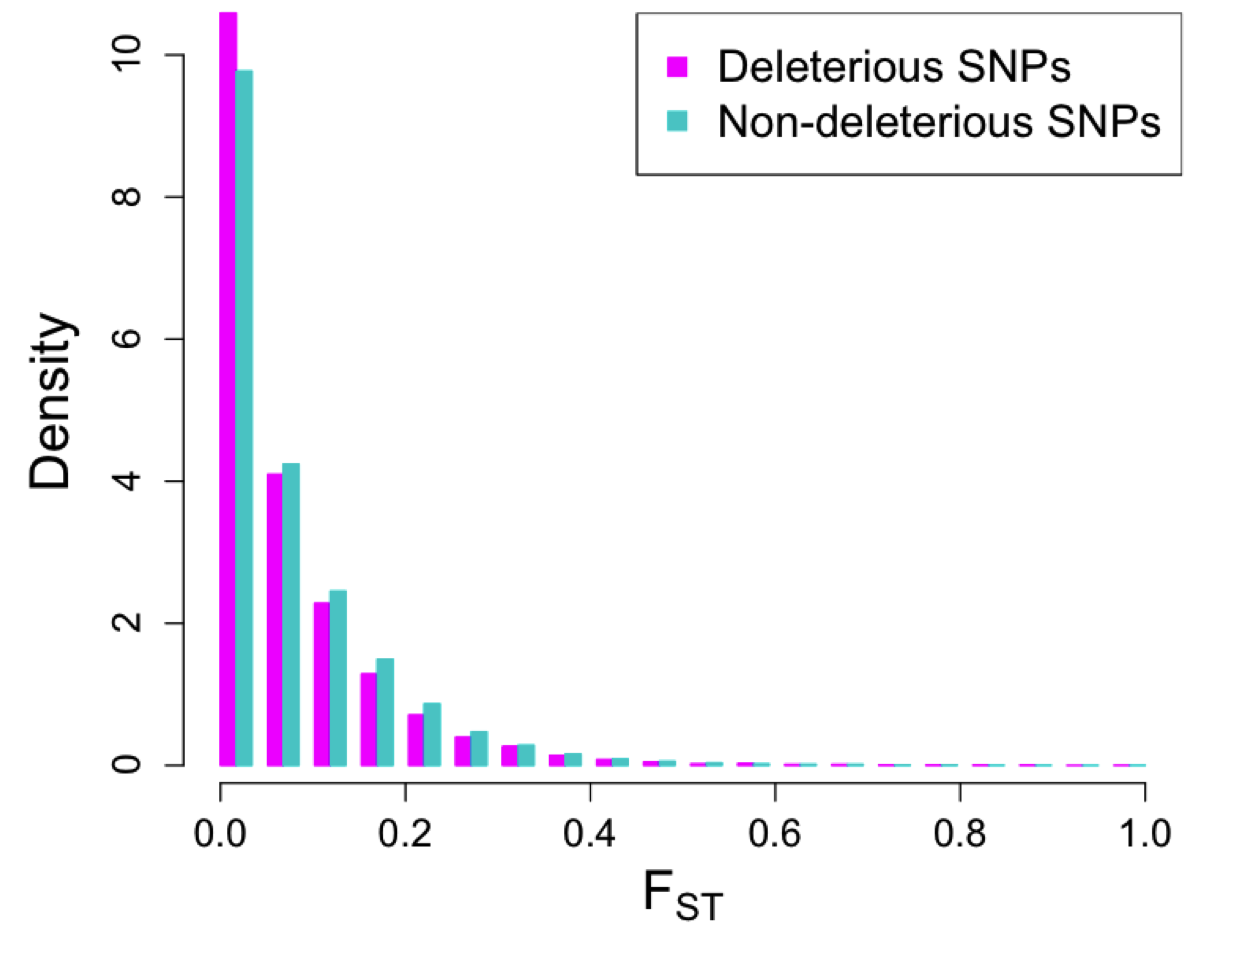
\includegraphics[width=90mm]{Fst.png}
    \caption{$\mathrm{F}_{\mathrm{ST}}$ distribution for deleterious and non-deleterious SNPs}
   \label{fst_dist}
  \end{center}
\end{figure*}
%-------------------------------------------------------------------

Across all groups, levels of population differentiation were slightly lower for deleterious (mean $\mathrm{F}_{\mathrm{ST}}=0.07$) than non-deleterious (mean $\mathrm{F}_{\mathrm{ST}}=0.08$) SNPs (\sme{Mann-Whitney U test p-value $< 2.2\ 10^{-16}$} ; Figure~\ref{fst_dist}). After correcting for allele frequencies in both classes, however, these differences disappeared, and  the proportion of deleterious SNPs in the top 1\% was not significantly different from the proportion observed for all SNPs in genic regions and for synonymous SNPs (\sme{Fisher's Exact Test p-value $= 0.15$ }).  \com{ would be good to have numbers of supp. table here.}  Nonetheless, several regions along the genome showed predicted deleterious SNPs that are significantly differentiated (controlling for allele frequency) among the different groups (Figure~\ref{fst_chr1}).


% Figure3
%-------------------------------------------------------------------
\begin{figure*}[ht]
  \begin{center}
   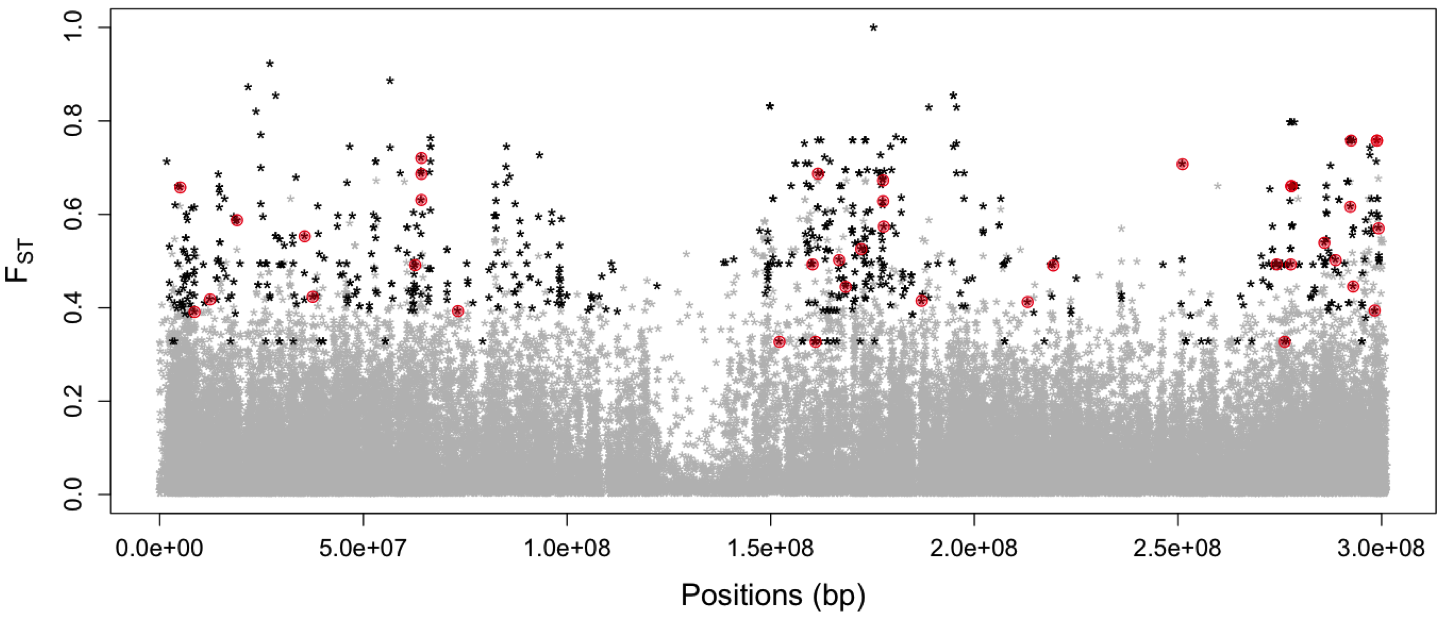
\includegraphics[width=150mm]{Fst2.png}
    \caption{$\mathrm{F}_{\mathrm{ST}}$ \com{is there a way to do the subscript without the italics? not sure.\smec{$\Rightarrow$done but may be a better way}} distribution along chromosome 1; black dots represent top 1\% SNPs, the predicted deleterious are surrounded in red.}\com{needs explanation of points/colors.  axis labels hard to read, and black/red points may need higher cex value?\smec{$\Rightarrow$figure changed}} 
   \label{fst_chr1}
  \end{center}
\end{figure*}
%-------------------------------------------------------------------

% Joint SFS

% Figure4
%-------------------------------------------------------------------
\begin{figure*}[ht]
  \begin{center}
   \includegraphics[width=110mm]{joinSFS.png}
    \caption{Joint site frequency spectrum of stiff-stalk, non stiff-stalk and tropical inbred lines}\com{SS NSS TS labels need to be bigger. gray "legend" box replaced with color legend.\smec{$\Rightarrow$done}}
   \label{jfs}
  \end{center}
\end{figure*}
%-------------------------------------------------------------------

Close comparisons of the site frequency spectrum of the predicted deleterious allele between stiff stalk, non stiff stalk, and tropical groups (Figure~\ref{jfs}) confirmed that most deleterious alleles are at low frequencies in \sme{all} groups compared and there were few fixed differences, but also revealed higher differentiation between the stiff stalk and the two other groups in comparison to the differentiation between the non stiff stalk and tropicals (Figure~\ref{jfs}). \com{what about JFS in pericentromeric regions? If fixation happens there faster (a la Gerke) then we might see something different? do we expect difference?\smec{$\Rightarrow$ nope! I had 727 SNPs in centremeric regions +/- 5 cM; the results doesn't show any obvious pattern}}

% along genome

% Figure5
%-------------------------------------------------------------------
\begin{figure*}[ht]
  \begin{center}
   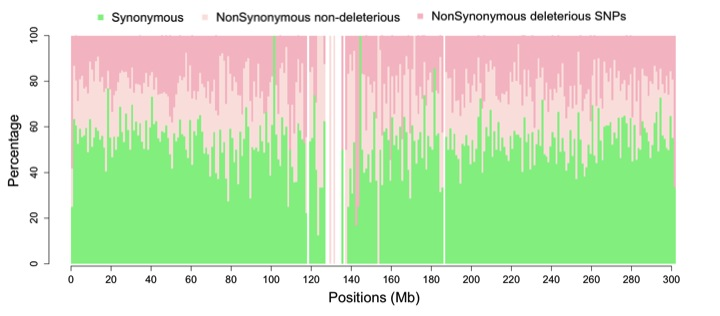
\includegraphics[width=140mm]{PerDelGenome_ch1.jpg}
    \caption{Distribution of synonymous, non-deleterious nonsynonymous and deleterious nonsynonymous SNPs along  chromosome 1} \com{love this figure.  can we change x label to simply "Mb" and y to "Percentage"\smec{$\Rightarrow$done}}
   \label{non_syn_chr1}
  \end{center}
\end{figure*}
%-------------------------------------------------------------------

\com{ this section is important and needs some intro. why do we expect correlations with recombination? why do we expect it to differ along the genome? I think we should also look at this -- i beleive you already ahve? -- within individual groups. }

Along the genome, as illustrated in Figure~\ref{non_syn_chr1} for the chromosome\,1, the percentage of SNPs with deleterious mutations in 1 Mega base pair windows, was uniform. Also, there was no correlation between the recombination rate and the percentage of deleterious SNPs observed. \com{ we need to check say �5cM around centromere compared to arms}

% -x-x-x-x-x-x-x-x-x-x-x-x-x-x-x-x-
\subsection*{Effect of deleterious mutations on traits of interest}
% -x-x-x-x-x-x-x-x-x-x-x-x-x-x-x-x-
In order to test the potential effect of the predicted deleterious variants, we performed a genome wide association mapping in the full panel using all available SNPs with a $MAF>0.05$. The analyses were carried out with \sme{both} the genetic values of inbred lines \sme{and hybrid vigor} to tests the effect of predicted deleterious mutations in inbreeding depression and heterosis.

Genome wide association results for inbred lines showed small but not significant enrichment for deleterious SNPs among significant associations (Table~\ref{table3} and Table~\ref{table4}). Nonetheless, we observed negative correlations between the number of deleterious SNPs associated with flowering time, plant morphology, seed number and seed weight and the genetic values of inbred lines (Table~\ref{table1} and Table~\ref{table2}). \com{GWAS associations is correct?\smec{I would prefere to avoid this abbreviation when talking about the results} you had amino acids coded by deleterious snps.\smec{$\Rightarrow$ yes; I did the correlations with both aa and SNPs}} These correlations are relatively high (Table~\ref{table3} and Table~\ref{table4}) \com{ho high?\smec{$\Rightarrow$ it's in the tables; should I put numbers here?}}, but should be interpreted with caution because the total number of significant SNPs is $<40$ in all cases.

Association mapping results of heterozygosity and heterosis showed variable numbers of significant loci (Table~\ref{table1} and Table~\ref{table2}). Virtually almost all traits exhibited a small enrichment (between $5$ and $45\%$) of deleterious SNPs among significant heterozygous associations, but only for whole plant yield and days to tasseling was the observed enrichment statistically significant. \com{ need to reduce number and complexity of tables.  should include what the \% enrichment was in text. did the enrichment tests account for multiple testing?\smec{$\Rightarrow$ No; but the associations holds when I control for the FDR at 10\%}}\\
Also, a moderately high correlation was observed, for several traits, between the number of heterozygote complementary alleles (one predicted  deleterious allele and one non deleterious) and hybrid vigor (Table~\ref{table3} and Table~\ref{table4}). \com{do these also show significant correlations with other SNP sets?} However, some of these correlations are not relevant because of the low number of significant loci observed. \com{I vote to not include these results.\smec{$\Rightarrow$ you mean al the correlation stuff or only the last sentence?}}

A number of factors likely contribute to the lack of enrichment seen in our results.  First, although we predicted $124,129$ SNPs, this is by no means a full accounting of the genic SNPs in the maize genome (see \citet{Chia2012} for comparison);  \sme{additionally, the predictions did not take into account the possible deleterious effects of SNPs in regulatory regions}. Second, our statistical power to evaluate deleterious alleles may be low.  The majority of the predicted deleterious SNPs are at low allele frequencies ($<5\%$) and cannot be included in the association analyses. \com{ i'm afraid a reviewer may ask us to do a burden test or some other test for rare alleles.  thoughts?\smec{$\Rightarrow$ if the question is asked, I will do it}} Moreover, under an additive model, deleterious mutations involved in heterosis are expected to have weak to intermediate effects, while deleterious mutations of large effect are likely to be purged from the population due to their effects on inbreeding depression  \citep{Charlesworth1987, Glemin2003, Charlesworth2009}. Combined, small effects and low allele frequency contributed to reduce our statistical power.

At a gene level, however, the enrichment of genes carrying deleterious SNPs within association mapping results was significant for heterosis observed in a non negligible part of the traits in population\,A (Table~\ref{table5}), which could be due to synthetic associations between rare causal deleterious loci and a common loci that reached an enough high frequent to be included in the association mapping analyses \citep{Dickson2010,Goldstein2009}. These enrichments did, however, not hold in population\,B mainly because of its small size (102 individuals).

 \com{ not sure what this is, but i think it needs expansion and explanation\smec{$\Rightarrow$The idea was that I have deleterious SNPs at low frequencies, I cannot test them but they are in LD with other tested SNPs in a given gene so it was an indirect way to check the enrichment for the deleterious SNPs that were not included in the GWAS; does it seem stupid/silly?}}

%----------------------------------------
% CONCLUSIONS
%----------------------------------------
\section*{Conclusion}
Using the reference B73 filtered gene set, we were able to carry out a maize whole genome scan for deleterious polymorphismes. Our prediction results, corroborated by theoretical expectations, showed a non negligible portion of deleterious SNPs segregating in the different heterotic groups with a higher percentage of shared deleterious alleles between inbred lines form the same heterotic group. Some of these deleterious alleles were shown to be significantly associated with the genetic values of inbred lines. We also showed a significant association of complementation at some of the deleterious alleles with hybrid vigor. 
The enrichment, in association mapping results, of significant deleterious SNPs was, as expected, not very high due to the small effect of deleterious SNPs that were not purged from the inbred population. However the enrichments were significant at a gene level. 

In the current study, we used a high density genotypic information to characterize deleterious SNPs in maize.  However, we were still missing a non negligible part of polymorphisms, including deleterious one. The full genome sequencing would thus allow the analyses of all segregating polymorphism. 
Also, we only focused the analyses on gene coding regions. Including regulatory regions and non-coding diversity in the deleterious effect estimate would be of interest.\\

%----------------------------------------
% ACKNOWLEGMENTS
%----------------------------------------
\subsubsection*{Acknowledgments}
We would like to thank S. Flint-Garcia for help with data analysis and G. Coop, J. Gerke, and P. Ralph for helpful comments. This project was supported by Agriculture and Food Research Initiative Competitive Grant 2009-01864 from the USDA�s National Institute of Food and Agriculture as well as a grant from DuPont Pioneer.
\\ \sme{Sho for his scripts for haplotype tests and different discussions we had }

%----------------------------------------
% REFERENCES
%----------------------------------------
\clearpage
\bibliography{Heterosis}



%----------------------------------------
% FIGURES AND TABLES
%----------------------------------------
\newpage
\section*{Tables}


%Table1
%-------------------------------------------------------------------
\begin{table*}[ht]
  \begin{center}
    \caption[]{Total number of significant SNPs (N. SNPs) and enrichment (Enri.), within genes, for loci with deleterious mutations in population\,A}
{\fontsize{10}{10}\sf
      \begin{tabular}{l|rr|rr|rr} 
\toprule
\multicolumn{1}{c}{}	&	\multicolumn{2}{c}{Inbreds}	&	\multicolumn{2}{c}{BPH}	&	\multicolumn{2}{c}{MPH}	\\	\hline 
Traits	& 	N.SNPs 	& 	Enri. 	& 	N.SNPs 	& 	Enri. 	& 	N.SNPs 	& 	Enri.	\\	\hline \hline 
DTT 	& 	475 	& 	1.05 	& 	3372 	& 	1.15* 	& 	1123 	& 	1.12	\\
TSLLEN 	& 	458 	& 	0.81 	& 	297 	& 	1.21 	& 	365 	& 	1.16	\\
TSLBCHCNT 	& 	300 	& 	0.98 	& 	4077 	& 	0.98 	& 	1257 	& 	1.12	\\
TSLANG 	& 	244 	& 	1.11 	& 	490 	& 	0.93 	& 	646 	& 	1.18	\\
PLTHT 	& 	282 	& 	0.92 	& 	18068 	& 	0.98 	& 	9712 	& 	0.93	\\
UPLFANG 	& 	415 	& 	1.20 	& 	8927 	& 	0.99 	& 	2266 	& 	1.12	\\
LFWDT 	& 	289 	& 	1.21 	& 	1064 	& 	1.16 	& 	1051 	& 	1.01	\\
LFLEN 	& 	389 	& 	1.14 	& 	4256 	& 	0.93 	& 	2257 	& 	1.07	\\
KNLHGT 	& 	292 	& 	1.10 	& 	8752 	& 	1.08 	& 	4512 	& 	1.01	\\
RPR 	& 	258 	& 	0.79 	& 	359 	& 	1.30 	& 	375 	& 	0.93	\\
PLTYLD 	& 	257 	& 	1.50 	& 	7440 	& 	1.12* 	& 	7007 	& 	1.14*	\\
EARLGH 	& 	231 	& 	0.89 	& 	605 	& 	1.11* 	& 	907 	& 	1.00	\\	
10KWT 	& 	298 	& 	1.29 	& 	709 	& 	1.15 	& 	761 	& 	1.30	\\
COBDIA 	& 	219 	& 	1.04 	& 	4363 	& 	1.16* 	& 	405 	& 	0.88	\\
COBWT 	& 	228 	& 	1.09 	& 	1746 	& 	0.93 	& 	519 	& 	0.69	\\
TOTKNLWT 	& 	256 	& 	0.88 	& 	3781 	& 	0.98 	& 	2045 	& 	0.95	\\
\bottomrule
      \end{tabular}
}
    \label{table1}  
  \end{center}
\end{table*}
%-------------------------------------------------------------------



%Table2
%-------------------------------------------------------------------
\begin{table*}[ht]
  \begin{center}
    \caption[]{Total number of significant SNPs (N. SNPs) and enrichment (Enri.), within genes, for loci with deleterious mutations in population\,B}
{\fontsize{9}{8}\sf
      \begin{tabular}{l|rr|rr|rr|rr|rr} 
\toprule
\multicolumn{1}{c}{}	&	\multicolumn{2}{c}{Inbreds}	&	\multicolumn{2}{c}{BPH\_B73}	&	\multicolumn{2}{c}{MPH\_B73}	&	\multicolumn{2}{c}{BPH\_Mo17}	&	\multicolumn{2}{c}{MPH\_Mo17}	\\	\hline 
Traits	& 	N.SNPs 	& 	Enri. 	& 	N.SNPs 	& 	Enri. 	& 	N.SNPs 	& 	Enri.	& 	N.SNPs 	& 	Enric. 	& 	N.SNPs 	& 	Enri.	\\	\hline \hline 
10KWT 	& 	310 	& 	0.77 	& 	404 	& 	1.17* 	& 	257 	& 	0.86 	& 	698 	& 	0.83 	& 	723 	& 	0.98	\\
COBWT 	& 	313 	& 	0.62 	& 	941 	& 	1.15* 	& 	387 	& 	0.69 	& 	257 	& 	1.33 	& 	532 	& 	0.95	\\
COBDIA 	& 	226 	& 	1.49 	& 	159 	& 	1.25* 	& 	236 	& 	1.06* 	& 	349 	& 	0.78 	& 	615 	& 	0.72	\\
COBLEN 	& 	598 	& 	1.08 	& 	239 	& 	1.20* 	& 	97 	& 	0.24 	& 	280 	& 	1.08 	& 	140 	& 	0.92	\\
SEEDWT 	& 	362 	& 	1.09 	& 	378 	& 	1.32* 	& 	118 	& 	1.23* 	& 	1043 	& 	0.92 	& 	1080 	& 	0.78	\\
SEEDNB 	& 	373 	& 	0.99 	& 	320 	& 	0.86 	& 	251 	& 	0.92 	& 	348 	& 	1.06 	& 	454 	& 	0.82	\\
PLTHT 	& 	505 	& 	1.02 	& 	261 	& 	0.89 	& 	143 	& 	1.45* 	& 	1022 	& 	1.08 	& 	156 	& 	1.16	\\
\bottomrule
      \end{tabular}
}
    \label{table2}  
  \end{center}
\end{table*}
%-------------------------------------------------------------------



%Table3
%-------------------------------------------------------------------
\begin{table*}[ht]
  \begin{center}
    \caption[]{Pearson coefficient of correlation of number of deleterious sites (All) or the number of significant ones (All sig.) with the different traits in population\,A}
{\fontsize{10}{10}\sf
      \begin{tabular}{l|rr|rr|rr} 
\toprule
\multicolumn{1}{c}{}	&	\multicolumn{2}{c}{Inbreds}	&	\multicolumn{2}{c}{BPH}	&	\multicolumn{2}{c}{MPH}	\\	\hline 
Traits 	& 	All 	& 	All sig. 	& 	All 	& 	All sig. 	& 	All 	& 	All sig.	\\ \hline \hline
DTT 	& 	0.17 	& 	-0.48 	& 	-0.07 	& 	-0.07 	& 	-0.58 	& 	-0.39	\\
TSLLEN 	& 	0.22 	& 	-0.07 	& 	0.36 	& 	0.22 	& 	0.54 	& 	0.25	\\
TSLBCHCNT 	& 	0.25 	& 	0.26 	& 	0.37 	& 	-0.02 	& 	0.19 	& 	-0.35	\\
TSLANG 	& 	-0.18 	& 	-0.45 	& 	-0.06 	& 	0.04 	& 	-0.18 	& 	-0.50	\\
PLTHT 	& 	-0.13 	& 	-0.30 	& 	0.40 	& 	0.19 	& 	0.51 	& 	0.27	\\
UPLFANG 	& 	-0.17 	& 	-0.53 	& 	0.46 	& 	0.45 	& 	-0.24 	& 	0.46	\\
LFWDT 	& 	0.06 	& 	-0.11 	& 	0.17 	& 	-0.01 	& 	0.27 	& 	0.29	\\
LFLEN 	& 	0.06 	& 	-0.03 	& 	0.36 	& 	-0.05 	& 	0.51 	& 	0.54	\\
KNLHGT 	& 	-0.29 	& 	-0.33 	& 	0.35 	& 	-0.23 	& 	0.52 	& 	0.32	\\
RPR 	& 	-0.01 	& 	0.25 	& 	-0.04 	& 	-0.47 	& 	-0.05 	& 	-0.05	\\
PLTYLD 	& 	-0.12 	& 	0.43 	& 	0.52 	& 	0.62 	& 	0.54 	& 	0.63	\\
EARLGH 	& 	-0.08 	& 	0.28 	& 	0.62 	& 	0.49 	& 	0.64 	& 	0.54	\\
10KWT 	& 	-0.06 	& 	0.25 	& 	0.25 	& 	0.33 	& 	0.32 	& 	0.65	\\
COBDIA 	& 	-0.18 	& 	0.08 	& 	0.14 	& 	-0.32 	& 	0.32 	& 	0.32	\\
COBWT 	& 	-0.18 	& 	0.18 	& 	0.48 	& 	0.07 	& 	0.58 	& 	0.50	\\
TOTKNLWT 	& 	-0.29 	& 	0.05 	& 	0.59 	& 	0.18 	& 	0.65 	& 	0.50	\\
\bottomrule
      \end{tabular}
}
    \label{table3}  
  \end{center}
\end{table*}
%-------------------------------------------------------------------



%Table4
%-------------------------------------------------------------------
\begin{table*}[ht]
  \begin{center}
    \caption[]{Pearson coefficient of correlation of number of deleterious sites (All) or the number of significant ones (All sig.) with the different traits in population\,B}
{\fontsize{10}{10}\sf
      \begin{tabular}{l|rr|rr|rr|rr|rr} 
\toprule
\multicolumn{1}{c}{}	&	\multicolumn{2}{c}{Inbreds}	&	\multicolumn{2}{c}{BPH\_B73}	&	\multicolumn{2}{c}{MPH\_B73}	&	\multicolumn{2}{c}{BPH\_Mo17}	&	\multicolumn{2}{c}{MPH\_Mo17}	\\	\hline 
Traits 	& 	All 	& 	All sig. 	& 	All 	& 	All sig. 	& 	All 	& 	All sig.	& 	All 	& 	All sig.	& 	All 	& 	All sig.	\\ \hline \hline
10KWT 	& 	-0.25 	& 	0.09 	& 	0.53 	& 	-0.24 	& 	0.53 	& 	-0.11 	& 	0.13 	& 	0.05 	& 	0.14 	& 	0.12	\\
COBWT 	& 	-0.17 	& 	-0.02 	& 	0.38 	& 	-0.15 	& 	0.43 	& 	0.65 	& 	0.18 	& 	0.36 	& 	0.14 	& 	0.56	\\
COBDIA 	& 	-0.21 	& 	0.07 	& 	0.22 	& 	0.51 	& 	0.27 	& 	0.65 	& 	0.23 	& 	-0.02 	& 	0.25 	& 	0.66	\\
COBLEN 	& 	0.15 	& 	0.57 	& 	0.34 	& 	-0.11 	& 	0.41 	& 	0.37 	& 	0.27 	& 	-0.40 	& 	0.26 	& 	-0.45	\\
SEEDWT 	& 	0.06 	& 	-0.35 	& 	0.18 	& 	-0.21 	& 	0.21 	& 	0.50 	& 	-0.08 	& 	0.18 	& 	-0.02 	& 	0.15	\\
SEEDNB 	& 	-0.32 	& 	-0.62 	& 	0.59 	& 	-0.20 	& 	0.56 	& 	0.02 	& 	0.21 	& 	-0.19 	& 	0.18 	& 	-0.02	\\
PLTHT 	& 	-0.25 	& 	-0.73 	& 	0.52 	& 	-0.02 	& 	0.60 	& 	0.53 	& 	0.00 	& 	-0.36 	& 	0.14 	& 	0.08	\\
\bottomrule
      \end{tabular}
}
    \label{table4}  
  \end{center}
\end{table*}
%-------------------------------------------------------------------



%Table5
%-------------------------------------------------------------------
\begin{table*}[ht]
  \begin{center}
    \caption[]{Total number of genes with significant SNPs (N. genes) and enrichment for genes with predicted deleterious SNPs(Enri.) in population\,A}
{\fontsize{10}{10}\sf
      \begin{tabular}{l|rr|rr|rr} 
\toprule
\multicolumn{1}{c}{}	&	\multicolumn{2}{c}{Inbreds}	&	\multicolumn{2}{c}{BPH}	&	\multicolumn{2}{c}{MPH}	\\	\hline 
Traits	& 	N.genes 	& 	Enri. 	& 	N.genes 	& 	Enri. 	& 	N.genes 	& 	Enri.	\\	\hline \hline 
DTT	&	176	&	1.11	&	1137	&	1.12*	&	429	&	1.15*		\\
TSLLEN	&	173	&	1.08	&	128	&	1.14	&	154	&	1.20	\\
TSLBCHCNT	&	114	&	1.02	&	1257	&	1.13*	&	472	&	1.14*		\\
TSLANG	&	103	&	1.03	&	177	&	1.10	&	254	&	1.15	\\
PLTHT	&	128	&	1.22	&	4529	&	1.10*	&	2741	&	1.10*	\\
UPLFANG	&	166	&	1.13	&	2553	&	1.11*	&	810	&	1.15*	\\
LFWDT	&	112	&	1.27	&	379	&	1.05	&	375	&	1.14	\\
LFLEN	&	141	&	1.18	&	1290	&	1.13*	&	821	&	1.20*	\\
KNLHGT	&	123	&	1.09	&	2633	&	1.13*	&	1506	&	1.14	\\
RPR	&	99	&	1.24	&	150	&	1.15	&	145	&	1.07	\\
PLTYLD	&	117	&	1.22	&	2440	&	1.14*	&	2302	&	1.14*		\\
EARLGH	&	84	&	1.02	&	230	&	1.20	&	333	&	1.15	\\
10KWT	&	137	&	1.18	&	288	&	1.17	&	308	&	1.13	\\
COBDIA	&	90	&	1.10	&	1419	&	1.13*	&	162	&	1.12	\\
COBWT	&	99	&	1.19	&	548	&	1.07	&	176	&	1.13	\\
TOTKNLWT	&	101	&	1.18	&	1228	&	1.11*	&	714	&	1.07	\\
\bottomrule
      \end{tabular}
}
    \label{table5}  
  \end{center}
\end{table*}
%-------------------------------------------------------------------



%Table6
%-------------------------------------------------------------------
\begin{table*}[ht]
  \begin{center}
    \caption[]{Total number of genes with significant SNPs (N. genes) and enrichment for genes with predicted deleterious SNPs(Enri.) in population\,B}
{\fontsize{10}{10}\sf
      \begin{tabular}{l|rr|rr|rr|rr|rr} 
\toprule
\multicolumn{1}{c}{}	&	\multicolumn{2}{c}{Inbreds}	&	\multicolumn{2}{c}{BPH\_B73}	&	\multicolumn{2}{c}{MPH\_B73}	&	\multicolumn{2}{c}{BPH\_Mo17}	&	\multicolumn{2}{c}{MPH\_Mo17}	\\	\hline 
Traits	& 	N.genes 	& 	Enri. 	& 	N.genes 	& 	Enri. 	& 	N.genes 	& 	Enri.	& 	N.genes 	& 	Enri. 	& 	N.genes 	& 	Enri.	\\	\hline \hline 
10KWT	&	73	&	1.17	&	169	&	1.14	&	95	&	1.11	&	246	&	1.11	&	274	&	1.11	\\
COBWT	&	71	&	1.13	&	316	&	1.08	&	128	&	1.04	&	94	&	1.10	&	204	&	1.10	\\
COBDIA	&	81	&	1.07	&	57	&	1.08	&	86	&	1.11	&	134	&	1.03	&	234	&	1.14	\\
COBLEN	&	203	&	1.09	&	89	&	1.24	&	30	&	1.17	&	110	&	1.17	&	51	&	1.21	\\
SEEDWT	&	138	&	1.10	&	146	&	1.14	&	50	&	0.97	&	371	&	1.09	&	389	&	1.09	\\
SEEDNB	&	106	&	1.15	&	128	&	1.13	&	116	&	0.98	&	130	&	1.12	&	166	&	1.09	\\
PLTHT	&	169	&	1.15	&	112	&	1.09	&	65	&	1.13	&	348	&	1.15	&	65	&	1.15	\\
\bottomrule
      \end{tabular}
}
    \label{table6}  
  \end{center}
\end{table*}
%-------------------------------------------------------------------




% -/\/\/\/\/\/\/\/\/\/\/\/\/\/\/\/\/\/\/\/\/\/\/\/\/\/\/\/\/\/\/\/\/\/\/\/\/\/\/\/\/\/\/\/\/\/\/\/\/\/\/\/\/\/\/\/\/\/\/\/\/\/\/\/\/\/\/\/\/\/\/\/\/\/\/\/\/\/\/\/\/\-
%  -X-X-X-X-X-X-X-X-X-X-X-X-X-X-X-X-X-X-X-X-X-X-X-X-X-X-X-X-X-X-X-X-X-X-X-X-X-X-X-X-X-X-X-X-X-X-
% -\/\/\/\/\/\/\/\/\/\/\/\/\/\/\/\/\/\/\/\/\/\/\/\/\/\/\/\/\/\/\/\/\/\/\/\/\/\/\/\/\/\/\/\/\/\/\/\/\/\/\/\/\/\/\/\/\/\/\/\/\/\/\/\/\/\/\/\/\/\/\/\/\/\/\/\/\/\/\/\/\/-

%----------------------------------------
% SUPPLEMENTALS
%----------------------------------------
\clearpage
\setcounter{figure}{0}
\setcounter{table}{0}
\renewcommand{\figurename}{Supp Fig.}
\renewcommand{\tablename}{Supp Table}

\section*{Supplementals}

\subsection*{List of the inbred lines used } 
\subsubsection*{ PopulationA}
B73, A214N, A441.5, A554, A556, A6, A619, A632, A634, A635, A641, A654, A659, A661, A679, A680, A682, AB28A, B10, B104, B105, B109, B115, B14A, B164, B2, B37, B46, B57, B64, B68, B73HTRHM, B75, B76, B77, B79, B84, B97, CH701.30, CH9, CI187.2, CI21E, CI28A, CI31A, CI3A, CI64, CI66, CI7, CI90C, CI91B, CM174, CM37, CM7, CML10, CML103, CML108, CML11, CML14, CML154Q, CML157Q, CML158Q, CML218, CML220, CML228, CML238, CML247, CML258, CML261, CML264, CML277, CML281, CML287, CML311, CML314, CML321, CML322, CML323, CML328, CML331, CML332, CML333, CML341, CML38, CML5, CML52, CML69, CML77, CML91, CML92, CMV3, CO255, D940Y, DE1, DE2, DE811, E2558W, EP1, F2834T, F44, F6, GA209, GT112, H105W, H84, H91, H95, H99, HI27, HP301, HY, I137TN, I205, I29, IA2132, IA5125, IDS28, IDS69, IDS91, IL101T, IL14H, IL677A, K148, K4, K55, K64, KI11, KI14, KI2021, KI21, KI3, KI43, KI44, KY21, KY226, KY228, L317, L578, M14, M162W, M37W, MEF156.55.2, MO17, MO18W, MO1W, MO24W, MO44, MO45, MO46, MOG, MP339, MS1334, MS153, MS71, MT42, N192, N28HT, N6, N7A, NC222, NC230, NC232, NC236, NC238, NC250, NC258, NC260, NC262, NC264, NC294, NC296, NC296A, NC298, NC300, NC302, NC304, NC306, NC310, NC314, NC318, NC320, NC324, NC326, NC328, NC33, NC336, NC338, NC342, NC344, NC346, NC348, NC350, NC352, NC354, NC356, NC358, NC360, NC362, NC364, NC366, NC368, ND246, OH40B, OH43E, OH603, OH7B, OS420, P39, PA762, PA875, PA880, PA91, R168, R177, R229, R4, SA24, SC357, SC55, SD44, SG1533, SG18, T232, T8, TX303, TZI10, TZI11, TZI16, TZI18, TZI25, TZI8, TZI9, U267Y, VA102, VA14, VA22, VA35, VA59, VA99, VAW6, W117HT, W153R, W182B, W64A, WD, X33.16, X38.11, X4226, X4722

\subsubsection*{ PopulationB}
B73, MO17, X33.16, A188, A239, A619, A632, A634, A635, A641, A654, A661, A679, A680, A682, B103, B104, B109, B115, B14A, B37, B46, B52, B57, B64, B68, B73, B73HTRHM, B75, B76, B77, B79, B84, C103, C49A, CH701.30, CM105, CM174, CO125, DE.2, DE1, DE811, EP1, H105W, H49, H84, H91, H95, H99, HP301, IL101, IL14H, K148, KY226, M14, MEF156.55.2, MO44, MO45, MO46, MO47, MS1334, MS153, MS71, N192, N28HT, N6, NC262, NC264, NC294, NC306, NC310, NC314, NC324, NC326, NC328, NC342, NC364, ND246, OH43, OH43E, OS420, P39, PA762, PA875, PA880, PA91, R168, R177, R4, SD40, SD44, SG18, VA102, VA14, VA17, VA22, VA35, VA85, VA99, W182B, W22, W64A, WF9, YU796.NS.


% FigureS1 
%-------------------------------------------------------------------
\begin{figure*}[h]
  \begin{center}
   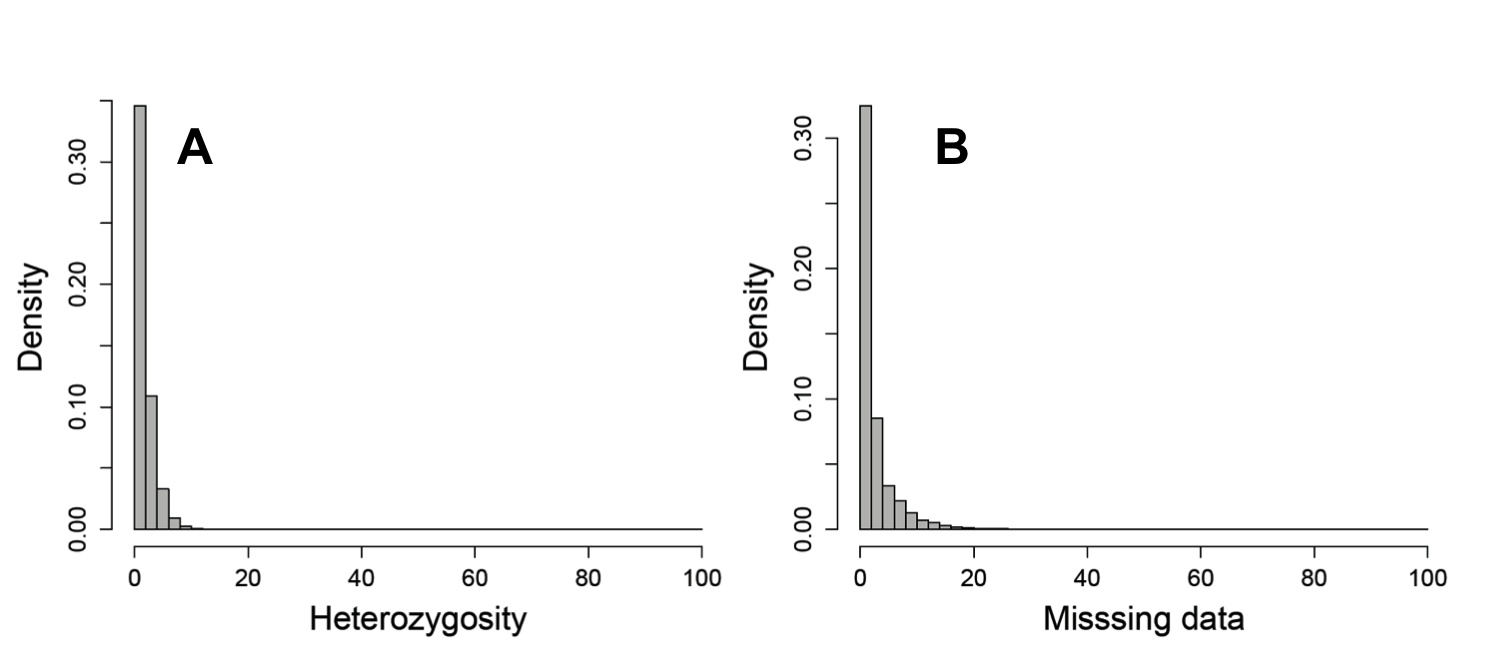
\includegraphics[width=150mm]{FigureS1.png}
    \caption{Histograms of the percentage of (A) heterozygosity and (B) missing data per SNP}
   \label{figureS1}
  \end{center}
\end{figure*}
%-------------------------------------------------------------------


\subsection*{List of genomes used for reciprocal BLAST}
\it{Aquilegia coerulea}, 
\it{Arabidopsis lyrata}, 
\it{Arabidopsis thaliana}, 
\it{Brachypodium distachyon}, 
\it{Brassica rapa}, 
\it{Capsella rubella}, 
\it{Carica papaya}, 
\it{Chlamydomonas reinhardtii}, 
\it{Citrus clementina}, 
\it{Citrus sinensis}, 
\it{Cucumis sativus}, 
\it{Eucalyptus grandis}, 
\it{Glycine max}, 
\it{Linum usitatissimum}, 
\it{Malus domestica}, 
\it{Manihot esculenta}, 
\it{Medicago truncatula}, 
\it{Mimulus guttatus}, 
\it{Oryza sativa}, 
\it{Panicum virgatum}, 
\it{Phaseolus vulgaris}, 
\it{Physcomitrella patens}, 
\it{Populus trichocarpa}, 
\it{Prunus persica}, 
\it{Ricinus communis}, 
\it{Selaginella moellendorffii}, 
\it{Setaria italica}, 
\it{Sorghum bicolor}, 
\it{Thellunigiella halophila}, 
\it{Vitis vinifera}, 
\it{Volvox carteri}.



%Table S1
%-------------------------------------------------------------------
\begin{table*}[ht]
{\fontsize{10}{10}\sf
\caption[]{Detailed results of the prediction of deleterious amino acids with MAPP, using the different gene sets, and with SIFT}
%  \textbf{}\\[-4mm]
\begin{tabular}{lrrrr} \hline
\toprule
\multicolumn{1}{c}{}	&	\multicolumn{3}{c}{MAPP}	&	\multicolumn{1}{c}{SIFT}	\\	\hline
Gene sets  & BLASTX & Reciprocal BLAST & Syntenic genes	&	PSI-BLAST \\	 \hline\hline
Total a.a. positions with predictions 	& 7,746,638 &	5,570,035 &	6,869,010	&	11,906,167 \\
Total number of genes &	20,348 &	11,918 &	17,957	&	31,843	\\
Number of positions covered by SNPs &	74,909 &	52,283 &	72,562	&	112,326	\\
Number of genes covered by SNPs &	12,561	&	8,553	&	12,615	&	19,145	\\
Monomorphic tolerated &	39,009 &	25,270 &	39,300	&	58,685	\\
Monomorphic not tolerated* &	144 &	3470 &	14	&	387	\\
Polymorphic tolerated	& 18,379 &	10,753 &		17,792	&	42,606	\\
Polymorphic not tolerated* &	 17,377 &	12,790 &	15456	&	10,648	\\
\bottomrule
\multicolumn{5}{l}{*Includes premature stop codons}
\end{tabular}
\label{tableS1}  % caption is needed to make this work
}
\end{table*}
%-------------------------------------------------------------------



%Table S2
%-------------------------------------------------------------------
\begin{table*}[ht]
  \begin{center}
    \caption[]{Comparion of the results of MAPP prediction with the different gene sets.} 
{\fontsize{10}{10}\sf
      \begin{tabular}{lccc}
\toprule
{Gene sets}		&	{      BLASTX      }	&	{      Reciprocal BLAST      }	&	{Syntenic genes}	\\ \hline \hline
BLASTX	&	-	&	80.1\%	&	78.2\%	\\
Reciprocal BLAST	&	38,054 (6,169)	&	-	&	79.8\%	\\
Syntenic genes		&	45,412 (7,745)	&	32,222 (5,488)	&	-	\\
\bottomrule
\multicolumn{4}{l}{The lower triangle indicates the number of  amino acid positions predicted with two given }	\\
\multicolumn{4}{l}{gene sets and covered by GBS SNPs (number of genes between brackets);  the upper }	\\
\multicolumn{4}{l}{triangle indicates the percentage of amino acids with the same predictions.}\\
      \end{tabular}
    \label{tableS2} 
}
  \end{center}
\end{table*}
%-------------------------------------------------------------------



% FigureS2 
%-------------------------------------------------------------------
\begin{figure*}[h]
  \begin{center}
   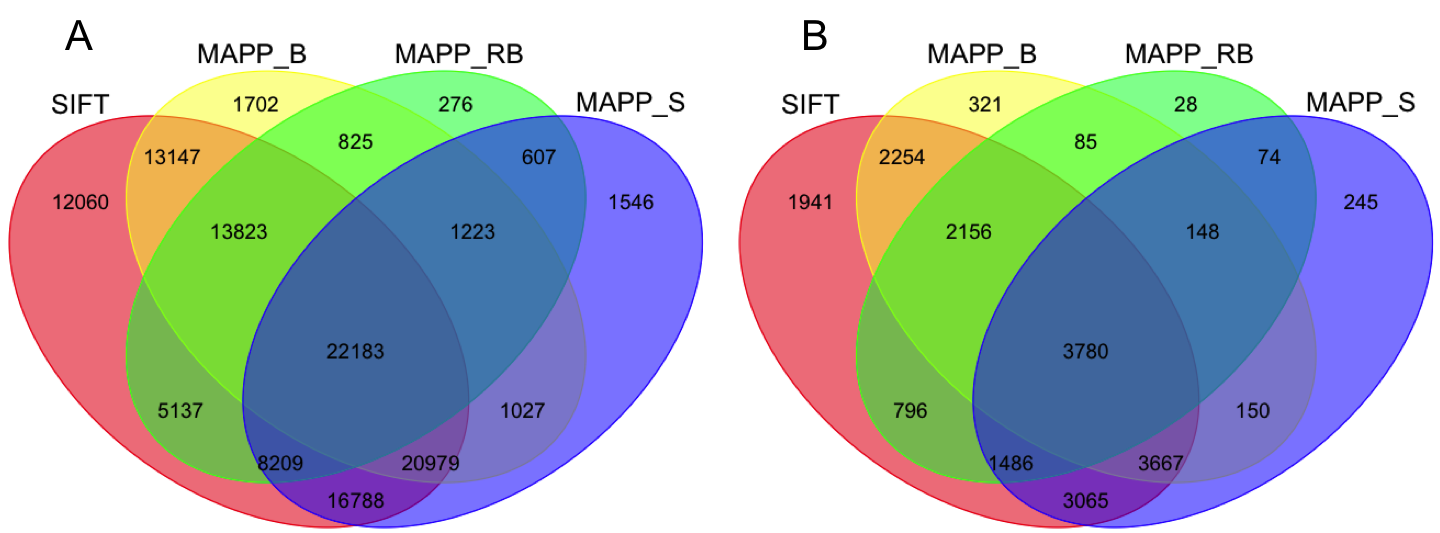
\includegraphics[width=150mm]{VennDiagram.png}
    \caption{Comparison of the number of predicted (A) amino acids and (B) genes, covered by SNP data. For MAPP, 3 gene sets were used: BLASTX (MAPP\_B), reciprocal BLAST (MAPP\_RB) and syntenic genes (MAPP\_S)}
   \label{figureS2}
  \end{center}
\end{figure*}
%-------------------------------------------------------------------


% FigureS3
%-------------------------------------------------------------------
\begin{figure*}[h]
  \begin{center}
   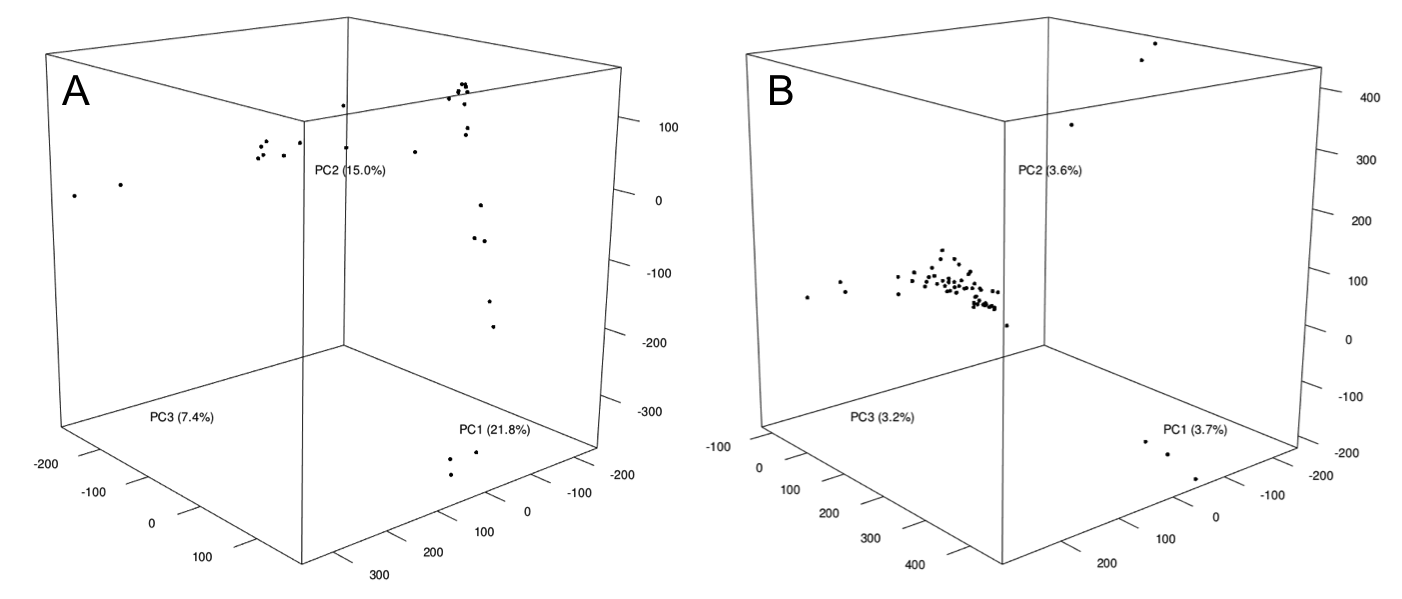
\includegraphics[width=150mm]{PCA.png}
    \caption{Projection of the (A) stiff stalk and (B) mixed inbred lines on the three first axes of a principal component analysis}
   \label{figureS3}
  \end{center}
\end{figure*}
%-------------------------------------------------------------------



\end{document}
%-----------------------------------------------------------------------------------------------------------------
%-----------------------------------------------------------------------------------------------------------------
% END DOCUMENT
%-----------------------------------------------------------------------------------------------------------------
%-----------------------------------------------------------------------------------------------------------------

% -/\/\/\/\/\/\/\/\/\/\/\/\/\/\/\/\/\/\/\/\/\/\/\/\/\/\/\/\/\/\/\/\/\/\/\/\/\/\/\/\/\/\/\/\/\/\/\/\/\/\/\/\/\/\/\/\/\/\/\/\/\/\/\/\/\/\/\/\/\/\/\/\/\/\/\/\/\/\/\/\/\-
%  -X-X-X-X-X-X-X-X-X-X-X-X-X-X-X-X-X-X-X-X-X-X-X-X-X-X-X-X-X-X-X-X-X-X-X-X-X-X-X-X-X-X-X-X-X-X-
% -\/\/\/\/\/\/\/\/\/\/\/\/\/\/\/\/\/\/\/\/\/\/\/\/\/\/\/\/\/\/\/\/\/\/\/\/\/\/\/\/\/\/\/\/\/\/\/\/\/\/\/\/\/\/\/\/\/\/\/\/\/\/\/\/\/\/\/\/\/\/\/\/\/\/\/\/\/\/\/\/\/-